\subsection{Diagrama Entidad-Relacion}
	\begin{figure}
	  \centering	
		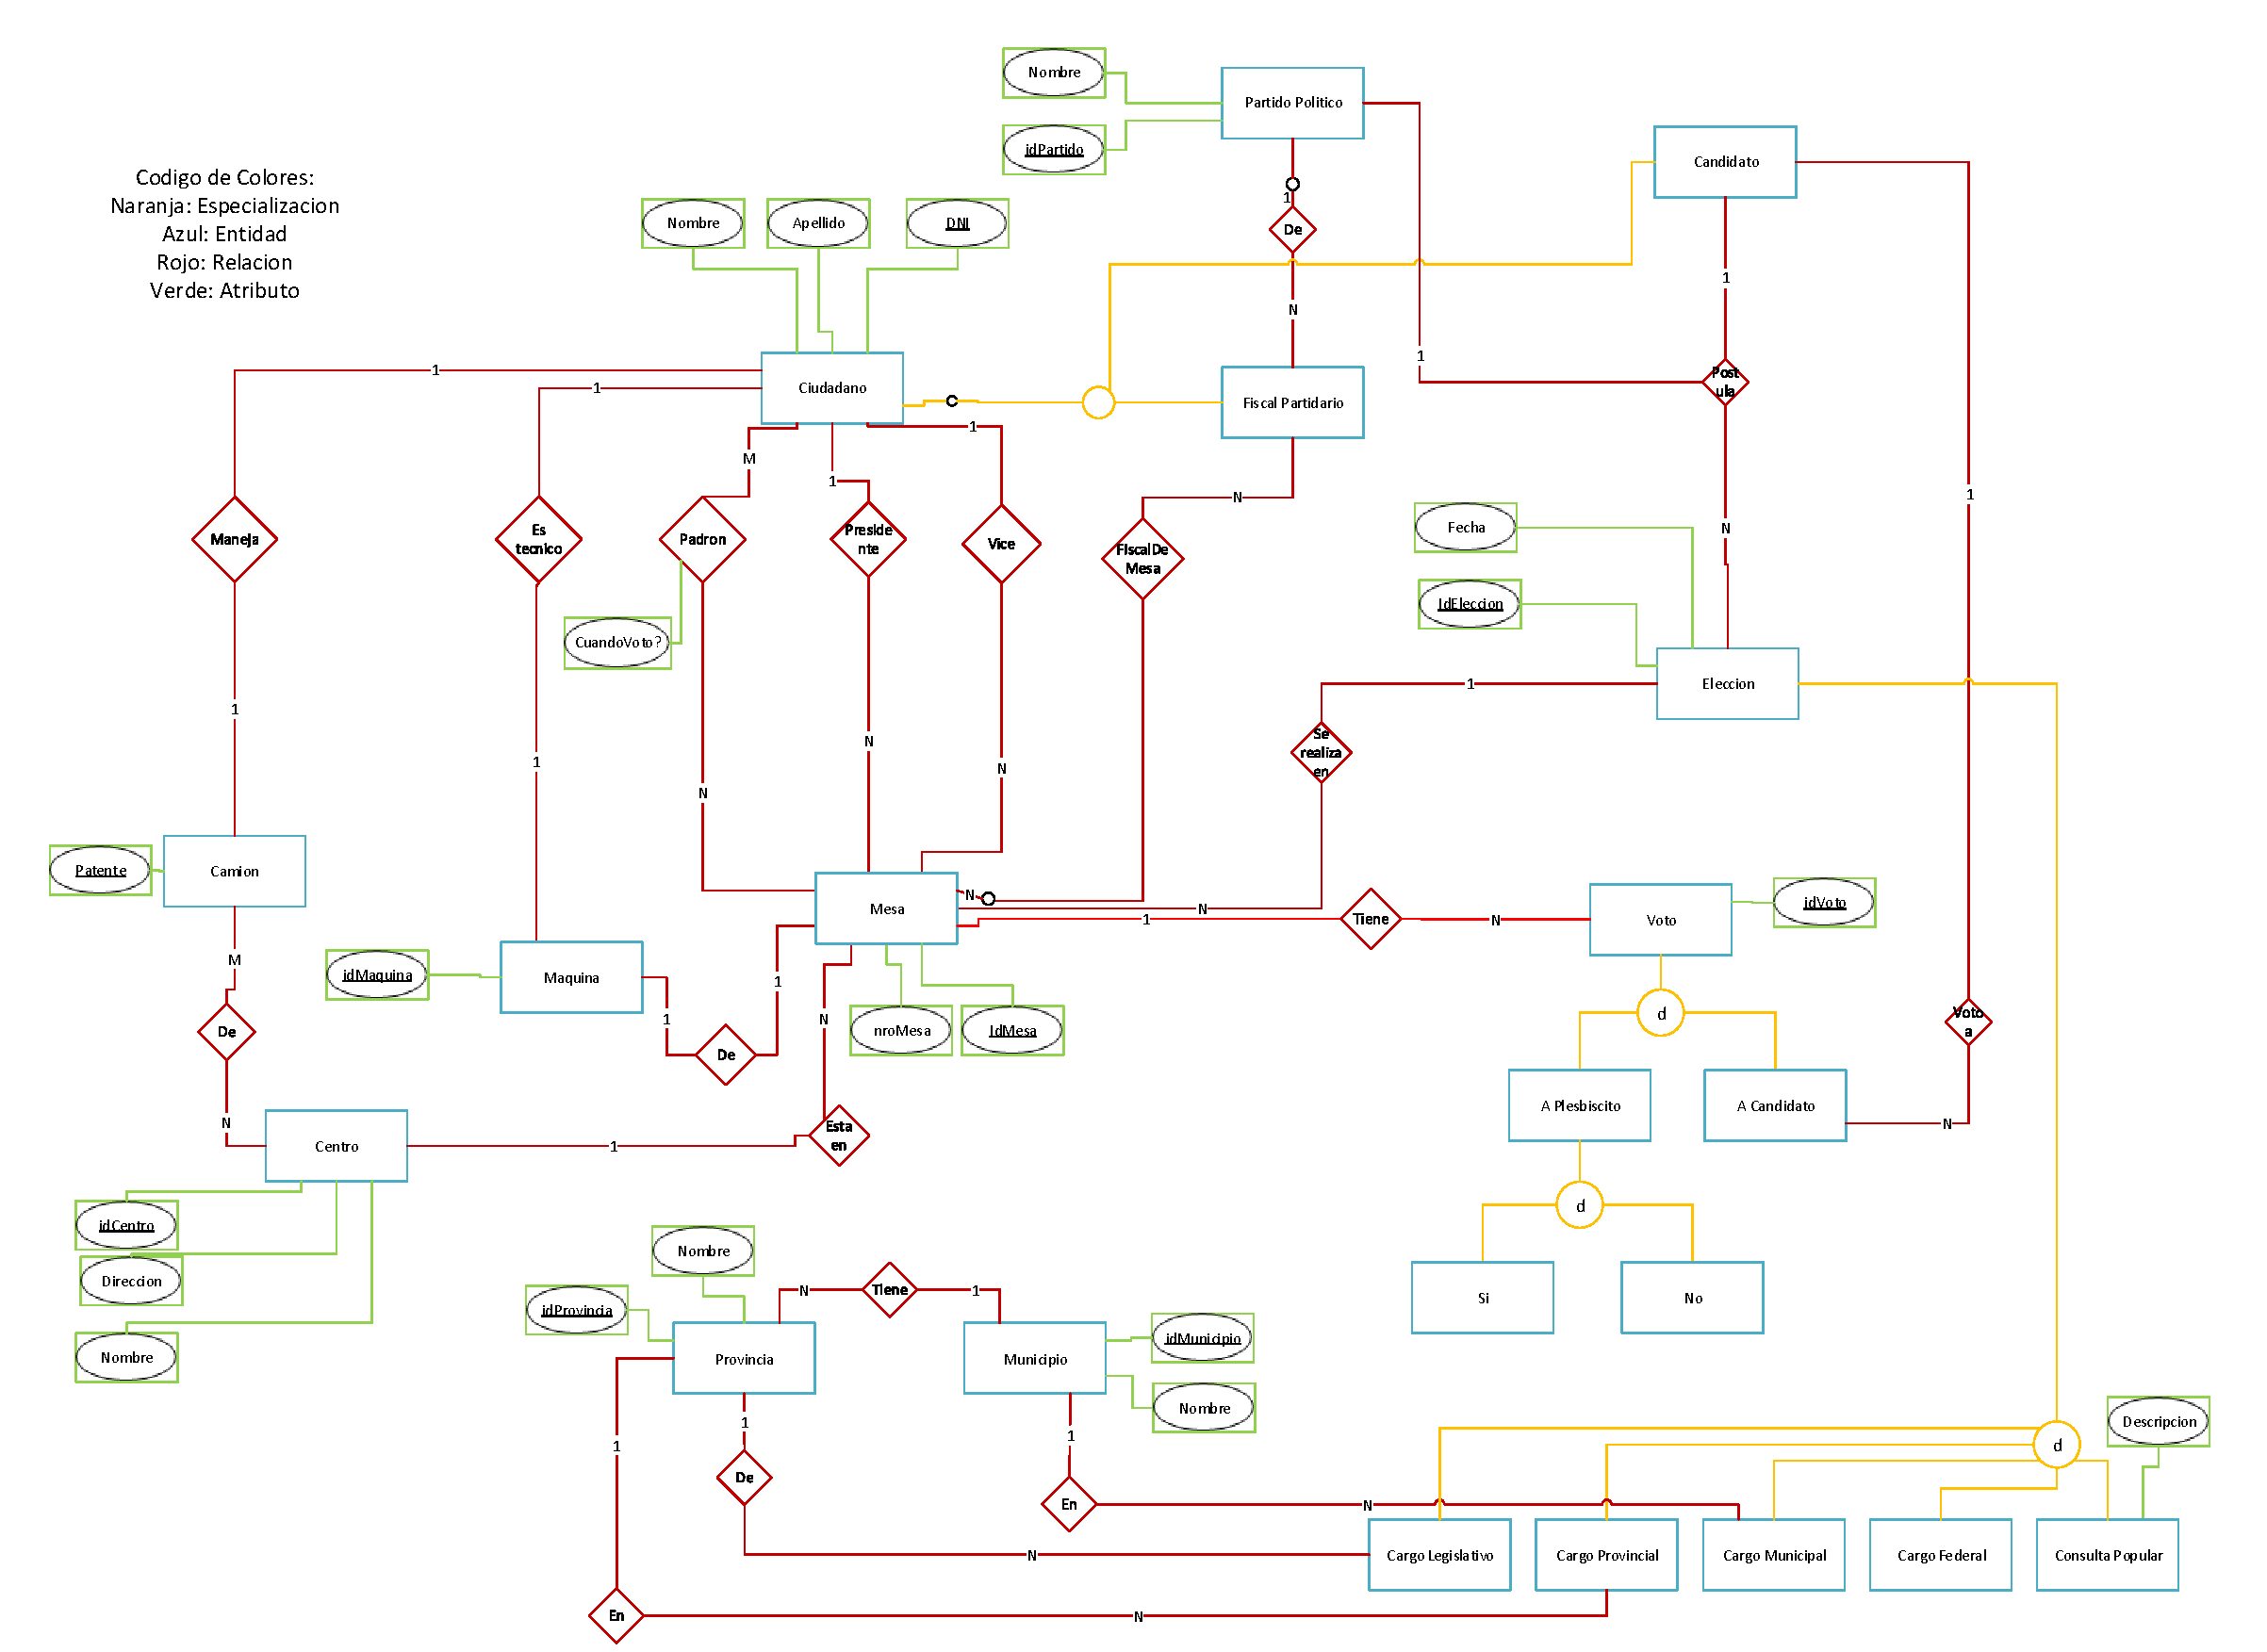
\includegraphics[scale=0.50]{fig/der.pdf}
	  \caption{Diagrama Entidad Relacion.}
	\end{figure}
\newpage

Restricciones Adicionales:

- Para cada persona que vota se debe insertar un voto(sin informacion de la persona) y actualizar correctamente la fecha y hora en la que voto y poniendo el “sello” virtual en el padron asignando un valor no nulo a cuandoVoto.

- La suma de los votos de todas las mesas de todos los candidatos debe ser menor o igual(votos en blanco diferencia) a la cantidad de ciudadanos que tiene el timestamp cuandoVoto? No nulo en el padron de dicha eleccion. (notar que esto tambien lo acota por la cantidad de ciudadanos)

- Todos los candidatos que se postulan para una eleccion, deben postularse para el mismo cargo.

- Asumimos que cada partido politico presenta un solo candidato.

- Los votos para una eleccion son: o bien consulta popular o bien de tipo candidato según corresponda el tipo de eleccion

-Si la eleccion es una consulta popular, los votos deben ser si/no. Sino, deben ser candidatos

-Un voto a candidato tiene que ser a un candidato que este postulado

- Un fiscal no puede estar en mas de una mesa en una eleccion

Habria que agregar como restriccion al der que un ciudadano no pueda ser tecnico, conductor, fiscal, etc en una misma eleccion.